%%%%%%%%%%%%%%%%%%%%%%%%%%%%%%%%%%%%%%%%%%%%%%%%%%%%%%%%%%%%%%%
%% OXFORD THESIS TEMPLATE

% Use this template to produce a standard thesis that meets the Oxford University requirements for DPhil submission
%
% Originally by Keith A. Gillow (gillow@maths.ox.ac.uk), 1997
% Modified by Sam Evans (sam@samuelevansresearch.org), 2007
% Modified by John McManigle (john@oxfordechoes.com), 2015
%
% This version Copyright (c) 2015-2023 John McManigle
%
% Broad permissions are granted to use, modify, and distribute this software
% as specified in the MIT License included in this distribution's LICENSE file.
%

% I've (John) tried to comment this file extensively, so read through it to see how to use the various options.  Remember
% that in LaTeX, any line starting with a % is NOT executed.  Several places below, you have a choice of which line to use
% out of multiple options (eg draft vs final, for PDF vs for binding, etc.)  When you pick one, add a % to the beginning of
% the lines you don't want.


%%%%% CHOOSE PAGE LAYOUT
% The most common choices should be below.  You can also do other things, like replacing "a4paper" with "letterpaper", etc.

% This one will format for two-sided binding (ie left and right pages have mirror margins; blank pages inserted where needed):
\documentclass[a4paper,twoside]{ociamthesis}
% This one will format for one-sided binding (ie left margin > right margin; no extra blank pages):
%\documentclass[a4paper]{ociamthesis}
% This one will format for PDF output (ie equal margins, no extra blank pages):
%\documentclass[a4paper,nobind]{ociamthesis} 



%%%%% SELECT YOUR DRAFT OPTIONS
% Three options going on here; use in any combination.  But remember to turn the first two off before
% generating a PDF to send to the printer!

% This adds a "DRAFT" footer to every normal page.  (The first page of each chapter is not a "normal" page.)
\fancyfoot[C]{\emph{DRAFT Printed on \today}}  

% This highlights (in blue) corrections marked with (for words) \mccorrect{blah} or (for whole
% paragraphs) \begin{mccorrection} . . . \end{mccorrection}.  This can be useful for sending a PDF of
% your corrected thesis to your examiners for review.  Turn it off, and the blue disappears.
\correctionstrue


%%%%% BIBLIOGRAPHY SETUP
% Note that your bibliography will require some tweaking depending on your department, preferred format, etc.
% The options included below are just very basic "sciencey" and "humanitiesey" options to get started.
% If you've not used LaTeX before, I recommend reading a little about biblatex/biber and getting started with it.
% If you're already a LaTeX pro and are used to natbib or something, modify as necessary.
% Either way, you'll have to choose and configure an appropriate bibliography format...

% The science-type option: numerical in-text citation with references in order of appearance.
\usepackage[style=numeric-comp, sorting=none, backend=biber, doi=false, isbn=false]{biblatex}
\newcommand*{\bibtitle}{References}

% The humanities-type option: author-year in-text citation with an alphabetical works cited.
%\usepackage[style=authoryear, sorting=nyt, backend=biber, maxcitenames=2, useprefix, doi=false, isbn=false]{biblatex}
%\newcommand*{\bibtitle}{Works Cited}

% This makes the bibliography left-aligned (not 'justified') and slightly smaller font.
\renewcommand*{\bibfont}{\raggedright\small}

% Change this to the name of your .bib file (usually exported from a citation manager like Zotero or EndNote).
\addbibresource{references.bib}


% Uncomment this if you want equation numbers per section (2.3.12), instead of per chapter (2.18):
%\numberwithin{equation}{subsection}



%%%%% THESIS / TITLE PAGE INFORMATION
% Everybody needs to complete the following:
\title{Suitably impressive thesis title}
\author{Your Name}
\college{Your College}

% Master's candidates who require the alternate title page (with candidate number and word count)
% must also un-comment and complete the following three lines:
%\masterssubmissiontrue
%\candidateno{933516}
%\wordcount{28,815}

% Uncomment the following line if your degree also includes exams (eg most masters):
%\renewcommand{\submittedtext}{Submitted in partial completion of the}
% Your full degree name.  (But remember that DPhils aren't "in" anything.  They're just DPhils.)
\degree{Doctor of Philosophy}
% Term and year of submission, or date if your board requires (eg most masters)
\degreedate{Michaelmas 2014}


%%%%% YOUR OWN PERSONAL MACROS
% This is a good place to dump your own LaTeX macros as they come up.

% To make text superscripts shortcuts
	\renewcommand{\th}{\textsuperscript{th}} % ex: I won 4\th place
	\newcommand{\nd}{\textsuperscript{nd}}
	\renewcommand{\st}{\textsuperscript{st}}
	\newcommand{\rd}{\textsuperscript{rd}}

%%%%% THE ACTUAL DOCUMENT STARTS HERE
\begin{document}



%%%%% CHOOSE YOUR LINE SPACING HERE
% This is the official option.  Use it for your submission copy and library copy:
\setlength{\textbaselineskip}{22pt plus2pt}
% This is closer spacing (about 1.5-spaced) that you might prefer for your personal copies:
%\setlength{\textbaselineskip}{18pt plus2pt minus1pt}

% You can set the spacing here for the roman-numbered pages (acknowledgements, table of contents, etc.)
\setlength{\frontmatterbaselineskip}{17pt plus1pt minus1pt}

% Leave this line alone; it gets things started for the real document.
\setlength{\baselineskip}{\textbaselineskip}


%%%%% CHOOSE YOUR SECTION NUMBERING DEPTH HERE
% You have two choices.  First, how far down are sections numbered?  (Below that, they're named but
% don't get numbers.)  Second, what level of section appears in the table of contents?  These don't have
% to match: you can have numbered sections that don't show up in the ToC, or unnumbered sections that
% do.  Throughout, 0 = chapter; 1 = section; 2 = subsection; 3 = subsubsection, 4 = paragraph...

% The level that gets a number:
\setcounter{secnumdepth}{2}
% The level that shows up in the ToC:
\setcounter{tocdepth}{2}


%%%%% ABSTRACT SEPARATE
% This is used to create the separate, one-page abstract that you are required to hand into the Exam
% Schools.  You can comment it out to generate a PDF for printing or whatnot.
\begin{abstractseparate}
	My abstract text goes here.  Check your departmental regulations, but generally this should be less than 300 words.  See the beginning of Chapter~\ref{ch:2-litreview} for more.

Lorem ipsum dolor sit amet, consectetur adipiscing elit. Pellentesque sit amet nibh volutpat, scelerisque nibh a, vehicula neque. Integer placerat nulla massa, et vestibulum velit dignissim id. Ut eget nisi elementum, consectetur nibh in, condimentum velit. Quisque sodales dui ut tempus mattis. Duis malesuada arcu at ligula egestas egestas. Phasellus interdum odio at sapien fringilla scelerisque. Mauris sagittis eleifend sapien, sit amet laoreet felis mollis quis. Pellentesque dui ante, finibus eget blandit sit amet, tincidunt eu neque. Vivamus rutrum dapibus ligula, ut imperdiet lectus tincidunt ac. Pellentesque ac lorem sed diam egestas lobortis.

Suspendisse leo purus, efficitur mattis urna a, maximus molestie nisl. Aenean porta semper tortor a vestibulum. Suspendisse viverra facilisis lorem, non pretium erat lacinia a. Vestibulum tempus, quam vitae placerat porta, magna risus euismod purus, in viverra lorem dui at metus. Sed ac sollicitudin nunc. In maximus ipsum nunc, placerat maximus tortor gravida varius. Suspendisse pretium, lorem at porttitor rhoncus, nulla urna condimentum tortor, sed suscipit nisi metus ac risus.

Aenean sit amet enim quis lorem tristique commodo vitae ut lorem. Duis vel tincidunt lacus. Sed massa velit, lacinia sed posuere vitae, malesuada vel ante. Praesent a rhoncus leo. Etiam sed rutrum enim. Pellentesque lobortis elementum augue, at suscipit justo malesuada at. Lorem ipsum dolor sit amet, consectetur adipiscing elit. Praesent rhoncus convallis ex. Etiam commodo nunc ex, non consequat diam consectetur ut. Pellentesque vitae est nec enim interdum dapibus. Donec dapibus purus ipsum, eget tincidunt ex gravida eget. Donec luctus nisi eu fringilla mollis. Donec eget lobortis diam.

Suspendisse finibus placerat dolor. Etiam ornare elementum ex ut vehicula. Donec accumsan mattis erat. Quisque cursus fringilla diam, eget placerat neque bibendum eu. Ut faucibus dui vitae dolor porta, at elementum ipsum semper. Sed ultrices dui non arcu pellentesque placerat. Etiam posuere malesuada turpis, nec malesuada tellus malesuada. % Create an abstract.tex file in the 'text' folder for your abstract.
\end{abstractseparate}


% JEM: Pages are roman numbered from here, though page numbers are invisible until ToC.  This is in
% keeping with most typesetting conventions.
\begin{romanpages}

% JEM: By default, this template uses the traditional Oxford "Belt Crest". Un-comment the following
% line to use the newer, "Blue Square" logo:
% \renewcommand{\crest}{{
\includegraphics[width=4.2cm, height=4.2cm]{figures/newlogo.pdf}}}

% Title page is created here
\maketitle

%%%%% DEDICATION -- If you'd like one, un-comment the following.
%\begin{dedication}
%This thesis is dedicated to\\
%someone\\
%for some special reason\\
%\end{dedication}

%%%%% ACKNOWLEDGEMENTS -- Nothing to do here except comment out if you don't want it.
\begin{acknowledgements}
 	\subsection*{Personal}

This is where you thank your advisor, colleagues, and family and friends.

Lorem ipsum dolor sit amet, consectetur adipiscing elit. Vestibulum feugiat et est at accumsan. Praesent sed elit mattis, congue mi sed, porta ipsum. In non ullamcorper lacus. Quisque volutpat tempus ligula ac ultricies. Nam sed erat feugiat, elementum dolor sed, elementum neque. Aliquam eu iaculis est, a sollicitudin augue. Cras id lorem vel purus posuere tempor. Proin tincidunt, sapien non dictum aliquam, ex odio ornare mauris, ultrices viverra nisi magna in lacus. Fusce aliquet molestie massa, ut fringilla purus rutrum consectetur. Nam non nunc tincidunt, rutrum dui sit amet, ornare nunc. Donec cursus tortor vel odio molestie dignissim. Vivamus id mi erat. Duis porttitor diam tempor rutrum porttitor. Lorem ipsum dolor sit amet, consectetur adipiscing elit. Sed condimentum venenatis consectetur. Lorem ipsum dolor sit amet, consectetur adipiscing elit.

Aenean sit amet lectus nec tellus viverra ultrices vitae commodo nunc. Mauris at maximus arcu. Aliquam varius congue orci et ultrices. In non ipsum vel est scelerisque efficitur in at augue. Nullam rhoncus orci velit. Duis ultricies accumsan feugiat. Etiam consectetur ornare velit et eleifend.

Suspendisse sed enim lacinia, pharetra neque ac, ultricies urna. Phasellus sit amet cursus purus. Quisque non odio libero. Etiam iaculis odio a ex volutpat, eget pulvinar augue mollis. Mauris nibh lorem, mollis quis semper quis, consequat nec metus. Etiam dolor mi, cursus a ipsum aliquam, eleifend venenatis ipsum. Maecenas tempus, nibh eget scelerisque feugiat, leo nibh lobortis diam, id laoreet purus dolor eu mauris. Pellentesque habitant morbi tristique senectus et netus et malesuada fames ac turpis egestas. Nulla eget tortor eu arcu sagittis euismod fermentum id neque. In sit amet justo ligula. Donec rutrum ex a aliquet egestas.

\subsection*{Institutional}

If you want to separate out your thanks for funding and institutional support, I don't think there's any rule against it.  Of course, you could also just remove the subsections and do one big traditional acknowledgement section.

Lorem ipsum dolor sit amet, consectetur adipiscing elit. Ut luctus tempor ex at pretium. Sed varius, mauris at dapibus lobortis, elit purus tempor neque, facilisis sollicitudin felis nunc a urna. Morbi mattis ante non augue blandit pulvinar. Quisque nec euismod mauris. Nulla et tellus eu nibh auctor malesuada quis imperdiet quam. Sed eget tincidunt velit. Cras molestie sem ipsum, at faucibus quam mattis vel. Quisque vel placerat orci, id tempor urna. Vivamus mollis, neque in aliquam consequat, dui sem volutpat lorem, sit amet tempor ipsum felis eget ante. Integer lacinia nulla vitae felis vulputate, at tincidunt ligula maximus. Aenean venenatis dolor ante, euismod ultrices nibh mollis ac. Ut malesuada aliquam urna, ac interdum magna malesuada posuere.
\end{acknowledgements}

%%%%% ABSTRACT -- Nothing to do here except comment out if you don't want it.
\begin{abstract}
	My abstract text goes here.  Check your departmental regulations, but generally this should be less than 300 words.  See the beginning of Chapter~\ref{ch:2-litreview} for more.

Lorem ipsum dolor sit amet, consectetur adipiscing elit. Pellentesque sit amet nibh volutpat, scelerisque nibh a, vehicula neque. Integer placerat nulla massa, et vestibulum velit dignissim id. Ut eget nisi elementum, consectetur nibh in, condimentum velit. Quisque sodales dui ut tempus mattis. Duis malesuada arcu at ligula egestas egestas. Phasellus interdum odio at sapien fringilla scelerisque. Mauris sagittis eleifend sapien, sit amet laoreet felis mollis quis. Pellentesque dui ante, finibus eget blandit sit amet, tincidunt eu neque. Vivamus rutrum dapibus ligula, ut imperdiet lectus tincidunt ac. Pellentesque ac lorem sed diam egestas lobortis.

Suspendisse leo purus, efficitur mattis urna a, maximus molestie nisl. Aenean porta semper tortor a vestibulum. Suspendisse viverra facilisis lorem, non pretium erat lacinia a. Vestibulum tempus, quam vitae placerat porta, magna risus euismod purus, in viverra lorem dui at metus. Sed ac sollicitudin nunc. In maximus ipsum nunc, placerat maximus tortor gravida varius. Suspendisse pretium, lorem at porttitor rhoncus, nulla urna condimentum tortor, sed suscipit nisi metus ac risus.

Aenean sit amet enim quis lorem tristique commodo vitae ut lorem. Duis vel tincidunt lacus. Sed massa velit, lacinia sed posuere vitae, malesuada vel ante. Praesent a rhoncus leo. Etiam sed rutrum enim. Pellentesque lobortis elementum augue, at suscipit justo malesuada at. Lorem ipsum dolor sit amet, consectetur adipiscing elit. Praesent rhoncus convallis ex. Etiam commodo nunc ex, non consequat diam consectetur ut. Pellentesque vitae est nec enim interdum dapibus. Donec dapibus purus ipsum, eget tincidunt ex gravida eget. Donec luctus nisi eu fringilla mollis. Donec eget lobortis diam.

Suspendisse finibus placerat dolor. Etiam ornare elementum ex ut vehicula. Donec accumsan mattis erat. Quisque cursus fringilla diam, eget placerat neque bibendum eu. Ut faucibus dui vitae dolor porta, at elementum ipsum semper. Sed ultrices dui non arcu pellentesque placerat. Etiam posuere malesuada turpis, nec malesuada tellus malesuada.
\end{abstract}

%%%%% MINI TABLES
% This lays the groundwork for per-chapter, mini tables of contents.  Comment the following line
% (and remove \minitoc from the chapter files) if you don't want this.  Un-comment either of the
% next two lines if you want a per-chapter list of figures or tables.
\dominitoc % include a mini table of contents
%\dominilof  % include a mini list of figures
%\dominilot  % include a mini list of tables

% This aligns the bottom of the text of each page.  It generally makes things look better.
\flushbottom

% This is where the whole-document ToC appears:
\tableofcontents

\listoffigures
	\mtcaddchapter
% \mtcaddchapter is needed when adding a non-chapter (but chapter-like) entity to avoid confusing minitoc

% Uncomment to generate a list of tables:
%\listoftables
%	\mtcaddchapter

%%%%% LIST OF ABBREVIATIONS
% This example includes a list of abbreviations.  Look at text/abbreviations.tex to see how that file is
% formatted.  The template can handle any kind of list though, so this might be a good place for a
% glossary, etc.
% List of abbreviations
\begin{mclistof}{List of Abbreviations}{3.2cm}
    \item[CHVI] Convex Hull Value Iteration.
    \item[CHVS] Convex Hull Value Set.
    \item[CMAB] Contextual Multi-Armed Bandit (problem).
    \item[CZ] Contextual Zooming. 
    \item[EMAB] Exploring Multi-Armed Bandit (problem).
    \item[MAB] Multi-Armed Bandit (problem). 
    \item[MCTS] Monte Carlo Tree Search.
    \item[\mctsone] A specific and common presentation of Monte Carlo Tree Search, presented in Section \ref{sec:2-4-thts}.
    \item[MDP] Markov Decision Process.
    \item[MENTS] Maximum ENtropy Tree Search.
    \item[MOMDP] Multi-Objective Markov Decision Process.
    \item[THTS] Trial-based Heuristic Tree Search.
    \item[\thtspp] An extension of THTS used in this thesis.
    \item[UCB] Upper Confidence Bound (algorithm).
    \item[UCT] Upper Confidence Bound applied to Trees.
\end{mclistof} 


% List of notation
\begin{mclistof}{List of Notation}{3.2cm}
    %%%%%
    % General Maths
    %%%%%
    \item[\Large\textbf{General Notation}\hfill\hfill]
    \item[$\one$] 
        The indicator function, where $\one(A)=1$ when $A$ is true, and $\one(A)=0$ when $A$ is false. 
    \item[$\hat{A}$] 
        The hat notation is used to denote an estimate, i.e. $\hat{A}$ is an estimate for some optimal value $A^*$
    \item[$\bar{A}$] 
        The bar notation is used to denote sample averages, i.e. $\bar{A}$ is a sample average of a number of samples $A_1,...,A_k$, or $\bar{A}=\frac{1}{n}\sum_{i=1}^k A_i$.
    \item[$\tilde{A}$] 
        The tilde notation is used to denote a function approximator, such as a neural network.
    \item[$\cl{A}$] 
        Calligraphic font is used to denote variables that are sets or tuples (ordered sets).
    \item[$\bff{A}$] 
        Bolt font is used to denote vectors, and $A_i$ is used to denote the $i$th component of the vector $\bff{A}$.
    \item[$\texttt{A}$]
        Typewriter text is used to refer to variables relating to an algorithm (or the analysis of an algorithm).
    \item[$\bfcl{A}$] 
        The notations above will also be combined at times, so $\bfcl{A}$ is used to denote a set that contains vectors.
    \item[$\bb{E}$] 
        The expectation operator. $\bb{E}[f]$ denotes the expectation of a distribution $f$, and $\bb{E}_{x\sim f}[g(x)]$ denotes the expected value of $g(x)$ under the distribution $f$.
    \item[$x\sim f$] 
        If $f:X\rightarrow[0,1]$ specifies a probability distribution, then $x\sim f$ denotes that the variable $x$ is sampled the distribution $f$.
    \\
    %%%%%
    % (MO)MDPs
    %%%%%
    \item[{\parbox[t]{\textwidth}{
            \Large\textbf{(Multi-Objective) Markov Decision Processes \\(Defined in Sections \ref{sec:2-2-mdps} and \ref{sec:2-5-morl})}\hfill\hfill
          }}]
    \item[$\cl{A}$]
        A (finite) set of actions.
    \item[$a_t$]
        The action at the $t$th timestep of a trajectory.
    \item[$D$]:
        The dimension of rewards in a MOMDP.
    \item[$H$]
        The finite-horizon time bound of an MDP.
    \item[$\cl{M}$]
        A Markov Decision Process, which is a tuple $\cl{M}=(\cl{S},s_0,\cl{A},R,p,H)$.
    \item[$\bfcl{M}$] 
        A Multi-Objective Markov Decision Process, which is a tuple $\bfcl{M}=(\cl{S},s_0,\cl{A},\bff{R},p,H)$.
    \item[$p$] 
        The next-state transition distribution of an MDP.  $p(s' | s,a) : \cl{S} \times \cl{A} \times \cl{S} \rightarrow [0,1]$.
    \item[$\pi$]:
        A policy, mapping a state $s\in\cl{S}$ to a probability distribution over actions $\cl{A}$.
        % \todo{probably dont need this, not going to use non-locally}
    \item[$R$] 
        The reward function of an MDP: $R(s,a) : \cl{S}\times \cl{A}\rightarrow \bb{R}$.
    \item[$\bff{R}$] 
        The $D$ dimensional reward function of a MOMDP: $\bff{R}(s,a) : \cl{S}\times \cl{A}\rightarrow \bb{R}^D$.
    \item[$r_t$]
        The reward at the $t$th timestep of a trajectory.
    \item[$\cl{S}$]
        A (finite) set of states.
    \item[$\suc{s}{a}$]
        The set of successor states of a state-action pair $(s,a)$, with respect to an MDP: $\suc{s}{a}=\{s'\in\cl{S}|p(s'|s,a)>0\}$.
    \item[$s_0$]
        $s_0\in\cl{S}$ is the initial starting state of an MDP.
    \item[$s_t$]
        The state at the $t$th timestep of a trajectory.
    \item[$\terminal(s)$]
        Denotes if a state $s$ is terminal or not. That is, if the transition distribution and reward function of the MDP is such that once reached, the state will never be left and no more reward will be received.
    \item[$\tau$]
        A trajectory, or sequence, of states, actions and rewards that are sampled according to a policy $\pi$ and an MDP $\cl{M}$: $\tau = (s_0, a_0, r_0, s_1, ..., s_{H-1}, a_{H-1}, r_{H-1}, s_H)$.
    \item[$\bff{\tau}$]
        A multi-objective trajectory, of states, actions and rewards that are sampled according to a policy $\pi$ and an MDP $\cl{M}$: $\bff{\tau} = (s_0, a_0, \bff{r}_0, s_1, ..., s_{H-1}, a_{H-1}, \bff{r}_{H-1}, s_H)$.
    % \item[$s,(s,a)\in\tau$] 
    %     \todo{define this here?} 
    \item[$\tau_{i:j}$]
        A truncated trajectory, starting at timestep $i$, and ending at timestep $j$: $\tau_{i:j} = (s_i, a_i, r_i, s_{i+1}, ..., s_{j-1}, a_{j-1}, r_{j-1}, s_j)$. 
    \item[$\bff{\tau}_{i:j}$] 
        A multi-objective truncated trajectory, starting at timestep $i$ and ending at timestep $j$: $\bff{\tau}_{i:j} = (s_i, a_i, \bff{r}_i, s_{i+1}, ..., s_{j-1}, a_{j-1}, \bff{r}_{j-1}, s_j)$.
    \\
    %%%%%
    % RL
    %%%%%
    \item[{\parbox[t]{\textwidth}{
            \Large\textbf{Reinforcement Learning (Section \ref{sec:2-3-rl})}\hfill\hfill
          }}]
    \item[$J(\pi)$] 
        The objective function for (standard) reinforcement learning: $J(\pi) = V^{\pi}(s_0;0)$.
    \item[$\pi^*$]
        The optimal standard policy, that maximises the objective function $J(\pi)$.
    \item[$Q^*$]
        The optimal Q-value function. $Q^*(s,a;t)$ denotes the maximal expected value that can be achieved by any policy, starting from state $s_t=s$, with action $a_t=a$.
    % \item[$\hat{Q}^k$]
    %     The estimate of the optimal value function after $k$ iterations of Value Iteration. 
    %     \todo{probably dont need this, not going to use non-locally}
    \item[$Q^{\pi}$]
        The Q-value function of a policy $\pi$. $Q^{\pi}(s,a;t)$ denotes the expected cumulative reward that policy $\pi$ will obtain, starting from state $s_t=s$, starting by taking action $a_t=a$.
    \item[$V^*$]
        The optimal value function. $V^*(s;t)$ denotes the maximal expected value that can be achieved by any policy, starting from state $s_t=s$.
    % \item[$\hat{V}^k$]
    %     The estimate of the optimal value function after $k$ iterations of Value Iteration.
    %     \todo{probably dont need this, not going to use non-locally}
    \item[$V^{\pi}$]
        The value of a policy $\pi$. $V^{\pi}(s;t)$ denotes the expected cumulative reward that policy $\pi$ will obtain, starting from state $s_t=s$.
    \\
    %%%%%
    % MERL
    %%%%%
    \item[{\parbox[t]{\textwidth}{
        \Large\textbf{Maximum Entropy Reinforcement Learning \\(Section \ref{sec:2-3-1-merl})}\hfill\hfill
      }}]
    \item[$\alpha$] 
        The temperature parameter, or, the coefficient of the entropy term in the maximum entropy (soft) objective.
    \item[$\cl{H}$]
        The Shannon entropy, of a probability distribution or policy.
    \item[$J_{\sft}(\pi)$] 
        The objective function for maximum entropy (soft) reinforcement learning: $J_{\sft}(\pi) = V_{\sft}^{\pi}(s_0;0)$.
    \item[$\pi_{\sft}^*$]
        The optimal soft policy, that maximises the soft objective function $J_{\sft}(\pi)$.
    \item[$Q_{\sft}^*$]
        The optimal soft Q-value function. $Q^*(s,a;t)$ denotes the maximal expected soft value that can be achieved by any policy, from state $s_t=s$ and taking action $a_t=a$. 
    \item[$Q_{\sft}^{\pi}$]
        The soft Q-value function of a policy $\pi$. $Q_{\sft}^{\pi}(s,a;t)$ is the expected value of the policy from $s_t=s$, starting with action $a_t=a$, with an addition of the entropy of the policy weighted by the temperature $\alpha$.
    \item[$V_{\sft}^*$]
        The optimal soft value function. $V^*(s;t)$ denotes the maximal expected soft value that can be achieved by any policy, from state $s_t=s$. 
    \item[$V_{\sft}^{\pi}$]
        The soft value of a policy $\pi$. $V_{\sft}^{\pi}(s;t)$ is the expected value of the policy from $s_t=s$, with an addition of the entropy of the policy weighted by the temperature $\alpha$.
    \\
    %%%%%
    % MORL
    %%%%%
    \item[{\parbox[t]{\textwidth}{
        \Large\textbf{Multi-Objective Reinforcement Learning \\(Section \ref{sec:2-5-morl})}\hfill\hfill
      }}]
    \item[$CCS(\Pi)$] 
        A convex coverage set of policies, which contains at least one policy that maximises the linear utility $u_{\lin}(\cdot;\bff{w})$ for each weight vector $\bff{w}$.
    \item[$CCS_{\min}(\Pi)$]
        The minimal convex coverage set of policies, which has no redundant policies and for each policy in $CCS_{\min}(\Pi)$ there is some weight that it uniquely (with respect to $CCS_{\min}(\Pi)$) obtains the optimal linear utility.
    \item[$CH(\Pi)$] 
        The undominated set of policies in $\Pi$ (the set of all possible policies), with respect to the linear utility function $u_{\lin}$. $CH(\Pi)=U(\Pi;u_{\lin})$.
    \item[$CS(\Pi;u)$] 
        A coverage set of policies, which contains at least one policy that maximises the utility $u(\cdot;\bff{w})$ for each weight vector $\bff{w}$.
    \item[$\cprune$] 
        An operation that takes an arbitrary set of vectors, and returns the subset that lie at the vertices of the geometric (partial) convex hull. 
    \item[$\Delta^D$] 
        The $D$ dimensional simplex, or, the set of possible weightings over the $D$ objectives of a MOMDP. $\Delta^D = \{\bff{w}\in\bb{R}^D|w_i > 0, \sum_i w_i = 1\}$.
    \item[$\Pi$] 
        The set of all possible policies in a MOMDP.
    \item[$\bff{Q}^{\pi}$]
        The multi-objective Q-value function of a policy $\pi$. $Q^{\pi}(s,a;t)$ denotes the expected cumulative vector reward that policy $\pi$ will obtain, starting from state $s_t=s$, starting by taking action $a_t=a$.
    \item[$U(\Pi;u)$] 
        The undominated set of policies in $\Pi$ (the set of all possible policies), with respect to the utility function $u$. Each policy in $U(\Pi;u)$ achieves a maximal utility for some weighting over the objectives.
    \item[$u$] 
        A utility function, mapping multi-objective values to scalar values, that depends on a weighting over objectives. The multi-objective value $\bff{V}^{\pi}(s,a;t)$ is mapped to $u(\bff{V}^{\pi}(s,a;t);\bff{w})$, where $\bff{w}$ is a weighting over the objectives.
    \item[$u_{\lin}$]
        The linear utility function: $u_{\lin}(\bff{v};\bff{w}) = \bff{w}^\top \bff{v}$.
    \item[$\bff{V}^{\pi}$]
        The multi-objective value of a policy $\pi$. $V^{\pi}(s;t)$ denotes the expected cumulative reward that policy $\pi$ will obtain, starting from state $s_t=s$.
    \item[$\valset(\Pi')$] 
        The set of multi-objective values obtained by a set of policies $\Pi'$.
    \item[$\bff{w}$] 
        A weighting over objectives that quantifies preferences over the multiple objectives, to be used in a utility function.
    \\
    %%%%%
    % THTS
    %%%%%
    \item[{\parbox[t]{\textwidth}{
        \Large\textbf{Trial Based Heuristic Tree Search (Section \ref{sec:2-4-thts})}\hfill\hfill
      }}]
    \item[$\backupv$]
        Updates the values at a decision node in the backup phase of a trial \thtspp, using the decision node's children, the trajectory sampled for the trial and the heuristic value function.
    \item[$\backupq$] 
        Updates the values at a chance node in the backup phase of a trial \thtspp, using the chance node's children, the trajectory sampled for the trial and the heuristic value function.
    \item[$H_{\thtspp}$]
        The planning horizon used in \thtspp, with $H_{\thtspp}\leq H$.
    \item[\mctsmode] 
        Specifies if \thtspp\ewe will sample a trajectory such that only one decision node is added to the search tree per trial. If not running in \mctsmode\ewe the \thtspp\ewe will sample a trajectory until the planning horizon $H_{\thtspp}$.
    \item[$N(s)$]
        The number of visits at the decision node corresponding to state $s$.
    \item[$N(s,a)$]
        The number of visits at the chance node corresponding to state-action pair $(s,a)$.
    \item[$\node(s)$] 
        The decision node corresponding to the state $s$.
    \item[$\node(s)\dotchildren$]
        The set of chance nodes that are children of $\node(s)$.
    \item[$\dnodedata{s}$]
        The set of variables stored at decision node $\node(s)$, typically used for estimating values.
    \item[$\node(s,a)$] 
        The chance node corresponding to the state-action pair $(s,a)$.
    \item[$\node(s,a)\dotchildren$]
        The set of decision nodes that are children of $\node(s,a)$.
    \item[$\cnodedata{s,a}$] 
        The set of variables stored at decision node $\node(s,a)$, typically used for estimating Q-values.
    \item[$\pisearch$]
        The search policy used in \thtspp\ewe to sample a trajectory in the selection phase.
    \item[$\Qinit$]
        The heuristic action function used in \thtspp, used to provide a Q-value estimate for any state-action pairs that aren't in the search tree.
    \item[$\samplecontext$]
        A function used in \thtspp\ewe that creates a context, or key-value story, and samples any initial values to be stored in the context.
    \item[$\sampleoutcome$]
        A function used in \thtspp\ewe to sample outcomes (successor states) from the environment (MDP).
    \item[$\cl{T}$] 
        The \thtspp\ewe search tree. $\cl{T}\subseteq \cl{S} \cup \cl{S}\times\cl{A}$. 
    \item[$\Vinit$]
        The heuristic value function used in \thtspp, used to initialise the value of a new decision node. 
    %
    %
    %
    % \\
    % %%%%%
    % % MABs
    % %%%%%
    % \item[\Large\textbf{Multi-Armed Bandits (Section \ref{sec:2-3-mab})}\hfill\hfill]
    % \item[$x$] \todo{define here and move into correct place in the list}
    % \item[$y$] \todo{define here and move into correct place in the list}
    % \item[$f_i$] \todo{define here and move into correct place in the list}
    % \item[$x^m$] \todo{define here and move into correct place in the list}
    % \item[$y^m$] \todo{define here and move into correct place in the list}
    % \item[$\bar{y}_i^m$] \todo{define here and move into correct place in the list}
    % \item[$N$] \todo{define here and move into correct place in the list}
    % \item[$\mu_i$] \todo{define here and move into correct place in the list}
    % \item[$\mu^*$] \todo{define here and move into correct place in the list}
    % \item[$\creg_{\mab}$] \todo{define here and move into correct place in the list}
    % \item[$\pi(m)$] \todo{define here and move into correct place in the list. Maybe keep it as this and ask question}
    % \item[$m$] \todo{define here and move into correct place in the list}
    % \item[$\pi_{\ucb}(m)$] \todo{define here and move into correct place in the list}
    % \item[$\pi^m$] \todo{define here and move into correct place in the list}
    % \item[$\psi^m$] \todo{define here and move into correct place in the list}
    % \item[$w$] \todo{define here and move into correct place in the list}
    % \item[$w^m$] \todo{define here and move into correct place in the list}
    % \item[$\mu_{w,i}$] \todo{define here and move into correct place in the list}
    % \item[$\mu_{w}^*$] \todo{define here and move into correct place in the list}
    % \item[$W$] \todo{define here and move into correct place in the list}
    % \item[$ $] \todo{define here and move into correct place in the list}
    % \item[$ $] \todo{define here and move into correct place in the list}
    % \item[$ $] \todo{define here and move into correct place in the list}
    % \item[$ $] \todo{define here and move into correct place in the list}
    %
    %
    %
    % \\
    % %%%%%
    % % UCT
    % %%%%%
    % \item[{\parbox[t]{\textwidth}{
    %     \Large\textbf{Upper Confidence Bound applied to Trees (Section \ref{sec:2-4-2-uct})}\hfill\hfill
    % }}]
    % \item[$\pirollout$] 
    %     A policy used to sample a trajectory that is used to estimate the value of a state being added to a search tree.
    % \item[$\piuct$] 
    %     The search policy used in UCT.
    % \item[$\Quct(s,a)$] 
    %     The sample-average value estimate used to estimate the Q-value at a chance node $(s,a)$ in UCT.
    % \item[$\hat{V}^{\pirollout}(s)$] 
    %     An estimate of $V^{\pirollout}(s)$ computed using the return from a single trajectory sampled using policy $\pirollout$. It is used to initialised the value of a state being added to the search tree.
    % \item[$\Vuct(s)$] 
    %     The sample-average value estimate used to estimate the value at a decision node $s$ in UCT. 
    %
    %
    %
    % \\
    % %%%%%
    % % MENTS
    % %%%%%
    % \item[{\parbox[t]{\textwidth}{
    %     \Large\textbf{Maximum ENtropy Tree Search (Section \ref{sec:2-4-3-ments})}\hfill\hfill
    % }}]
    % \item[$\alpha_{\ments}$] 
    %     The temperature parameter used in MENTS, which is the coefficient of the entropy terms in the maximum entropy objective.
    % \item[$\epsilon$]
    %     An exploration parameter used in MENTS.
    % \item[$\lambda_s$] 
    %     An exploration parameter used in MENTS.
    % \item[$\tilde{\pi}$] 
    %     A policy (neural) network, used to initialise soft Q-value estimates in MENTS, if available. 
    % \item[$\piments$] 
    %     The search policy used in MENTS.
    % \item[$\Qments(s,a)$] 
    %     A soft Q-value estimate at the chance node $(s,a)$ in MENTS.
    % \item[$\tilde{V}$] 
    %     A function approximation to $V^*$.
    % \item[$\Vments(s)$] 
    %     A soft value estimate at the decision node $s$ in MENTS.
\end{mclistof} 


% The Roman pages, like the Roman Empire, must come to its inevitable close.
\end{romanpages}


%%%%% CHAPTERS
% Add or remove any chapters you'd like here, by file name (excluding '.tex'):
\flushbottom
% \begin{savequote}[8cm]
% \textlatin{Neque porro quisquam est qui dolorem ipsum quia dolor sit amet, consectetur, adipisci velit...}

% There is no one who loves pain itself, who seeks after it and wants to have it, simply because it is pain...
%   \qauthor{--- Cicero's \textit{de Finibus Bonorum et Malorum}}
% \end{savequote}

\chapter{\label{ch:1-intro}Introduction} 

    \minitoc

    \todo{chapter structure (i.e. in the introduction section I give some background in the field(s), cover the main 
    contributions of this thesis, etc, etc).}

\section{Overview}
\label{sec:1-1-overview}

    \todo{list}
    \begin{itemize}
        \item Give some context around MCTS (and talk about exploration and exploitation), and why we might use it
        \begin{itemize}
            \item Larger scale than tabular methods
            \item Can do probability and theory stuff (and some explainability, by looking at stats in the tree the agent used)
            \item Can use tree search with neural networks to get some of the above (and use for neural network training as in alpha zero)
        \end{itemize}
        \item Argument from DENTS paper for exploration > exploitation (in context of planning in a simulator)
        \item Give high level overview of Multi-Objective RL, and why it can be useful
        \item Give an idea of how my work fits into MCTS and MORL as a whole
        \item Discuss research questions/issues with current literature (i.e. introduce some of the ideas from contributions section below)
    \end{itemize}

\section{Contributions}
\label{sec:1-2-contributions}

    \todo{Inline acronyms used, or make sure that they're defined before hand}

    Throughout this thesis, we will consider the following questions related to Monte Carlo Tree Search and Multi-Objective Reinforcement Learning:
    \begin{enumerate}[start=1, label={\textbf{Q\arabic* -}}]
        % \item \hypertarget{q1}{\textbf{Time-Limited Planning:}} How do we ensure that MCTS algorithms make good decisions when limited planning time is available?
        \item \hypertarget{q1}{\textbf{Exploration:}} When planning in a simulator with limited time, how can MCTS algorithms best explore to make good decisions?
        
        \begin{enumerate}[start=1, label={\textbf{Q1.\arabic* -}}]
            \item \hypertarget{q11}{\textbf{Entropy:}} Entropy is often used as an exploration objective in RL, but can it be used soundly in MCTS?
            \item \hypertarget{q12}{\textbf{Multi-Objective Exploration:}} How can Multi-Objective MCTS methods explore to find optimal actions for different objectives? 
        \end{enumerate}

        \item \hypertarget{q2}{\textbf{Scalability:}} How can the scalability of (multi-objective) MCTS methods be improved?

        \begin{enumerate}[start=1, label={\textbf{Q2.\arabic* -}}]
            \item \hypertarget{q21}{\textbf{Complexity:}} MCTS algorithms typically run in $O(nAH)$, but are there algorithms that can improve upon this?
            \item \hypertarget{q22}{\textbf{Multi-Objective Scalability:}} With respect to the size of environments, how scalable are Multi-Objective MCTS methods?
            \item \hypertarget{q23}{\textbf{Curse of Dimensionality:}} With respect to the number of objectives, to what extent do Multi-Objective MCTS methods suffer from the curse of dimensionality?
        \end{enumerate}


        \item \hypertarget{q3}{\textbf{Evaluation:}} How can we best evaluate a search tree produced by a Monte Carlo Tree Search algorithm?
        
        \begin{enumerate}[start=1, label={\textbf{Q3.\arabic* -}}]
            \item \hypertarget{q31}{\textbf{Tree Policies:}} Does it suffice to extract a policy from a single search tree for evaluation? \todo{going to have to run some extra experiments for that, but I probably should do that for completeness anyway}
            \item \hypertarget{q32}{\textbf{Multi-Objective Evaluation:}} Can we apply methods from the MORL literature to theoretically and empirically evaluate Multi-Objective MCTS?
        \end{enumerate}
    \end{enumerate}

    \todo{some words about how below is the contributions we're making in this thesis and expand these bullets a bit more}
    \begin{itemize}
        \item Max Entropy can be misaligned with reward maximisation (\entropyq)
        \item Boltzmann Search Policies - BTS and DENTS (\entropyq, and with extra results \treepolicyq)
        \item Use the alias method to make faster algorithms (\complexityq)
        \item Simple regret (\exploreq)
        \item Use of contexts in THTS to make consistent decisions in each trial (\contextq)
        \item Contextual regret introduced in CHMCTS (\moscalabilityq, \moevalq)
        \item Contextual Zooming and CHMCTS (designed for \contextq, runtimes cover \dimq, results \moevalq)
        \item Simplex maps (\contextq, \moscalabilityq, \dimq)
        \item Contextual Simple Regret (\moevalq)
    \end{itemize}

    \hide{\todo{Would like to do the comparing different types of eval, even if not listing it as a research question 
    (compare giving it X seconds per decision and evaluating that policy (SLOW), and comparing policy extracted from 
    the tree)}}

    \hide{\todo{can make an argument that the best bound achieved by theory is given by letting temperature go to max. Which is consistent with the exploring bandits results}}



\section{Structure of Thesis}
\label{sec:1-3-thesis-structure}

    \todo{a paragraph with a couple lines to a paragraph about each chapter. This is the high level overview/intro to 
    the thesis paragraph. I.e. this section is ``this is the story of my thesis in a page or two''}

\section{Publications}
\label{sec:1-4-publications}

    \todo{update final publication when submit}

    The work covered in this thesis also appears in the following publications:
    \begin{itemize}
        \item Painter, M; Lacerda, B; and Hawes, N. ``Convex Hull Monte-Carlo Tree-Search." In \textit{Proceedings of the international conference on automated planning and scheduling. Vol. 30. 2020}, ICAPS, 2020.
        \item Painter, M; Baioumy, M; Hawes, N; and Lacerda, B.  ``Monte Carlo Tree Search With Boltzmann Exploration." In \textit{Advances in Neural Information Processing Systems, 36, 2023}, NeurIPS, 2023.
        \item Painter, M; Hawes, N; and Lacerda, B. ``Simplex Maps for Multi-Objective Monte Carlo Tree Search." In \textit{TODO}, \textbf{Under Review at conf\_name}.
    \end{itemize}
\begin{savequote}[8cm]
Alles Gescheite ist schon gedacht worden.\\
Man muss nur versuchen, es noch einmal zu denken.

All intelligent thoughts have already been thought;\\
what is necessary is only to try to think them again.
  \qauthor{--- Johann Wolfgang von Goethe \cite{von_goethe_wilhelm_1829}}
\end{savequote}

\chapter{\label{ch:2-litreview}Background}

\minitoc

\section{Introduction}

This document introduction won't serve as a complete primer on \LaTeX.  There are plenty of those online, and googling your questions will often get you answers, especially from \url{http://tex.stackexchange.com}.

Instead, let's talk a little about a few of the features and packages lumped into this template situation.  The \verb|savequote| environment at the beginning of chapters can add some wittiness to your thesis.  If you don't like the quotes, just remove that block.

For when it comes time to do corrections, there are two useful commands here.  First, the \verb|mccorrect| command allows you to highlight a short correction \mccorrect{like this one}.  When the thesis is typeset normally, the correction will just appear as part of the text.  However, when you declare \verb|\correctionstrue| in the main \verb|Oxford_Thesis.tex| file, that correction will be highlighted in blue.  That might be useful for submitting a post-viva, corrected copy to your examiners so they can quickly verify you've completed the task.

\begin{mccorrection}
For larger chunks, like this paragraph or indeed entire figures, you can use the \verb|mccorrection| environment.  This environment highlights paragraph-sized and larger blocks with the same blue colour.
\end{mccorrection}

Read through the \verb|Oxford_Thesis.tex| file to see the various options for one- and two-sided printing, including or excluding the separate abstract page, and turning corrections and draft footer on or off, and the separate option to centre your text on the page (for PDF submission) or offset it (for binding).  There is also a separate option for master's degree submissions, which changes identifying information to candidate number and includes a word count.  (Unfortunately, \LaTeX has a hard time doing word counts automatically, so you'll have to enter the count manually if you require this.)

\section{Cardiac Imaging}\label{app:imaging}

Within months of Röntgen's discovery of the X-ray in \mccorrect{1895}\cite{gagliardi_rontgen_1996}, cardiac pathology was being investigated via non-invasive imaging \cite{gagliardi_cardiac_1996}.  Over the intervening years, cardiac imaging modalities and techniques have advanced significantly.  Clinically, cardiac imaging is used for two broad purposes: diagnosis of pathophysiology and guidance of interventional procedures.  These applications impose different requirements on imaging equipment, image acquisition time, computational complexity, spatial and temporal resolution, and tissue discrimination.  The common diagnostic and interventional cardiac imaging techniques in current clinical practice are reviewed below.  An accessible introduction to the physics of medical imaging can be found in Webb's \textit{Introduction to Biomedical Imaging} \cite{webb_introduction_2002}.  A comprehensive overview of the use of imaging in clinical cardiology is presented in Leeson's \textit{Cardiovascular Imaging} \cite{leeson_cardiovascular_2011}.

\subsection{Diagnostic Imaging}
\label{sub:diagnostic}

Beyond the chest X-ray (`plain film'), the key non-invasive imaging modalities in diagnostic cardiology are echocardiography, magnetic resonance imaging, and X-ray computed tomography, which are reviewed below.  Nuclear medicine, including positron emission tomography (PET) and single-photon emission computed tomography (SPECT), are not discussed here, as they do not play a role in the chapters to follow.

\subsubsection{Echocardiography}

\begin{figure}
\centering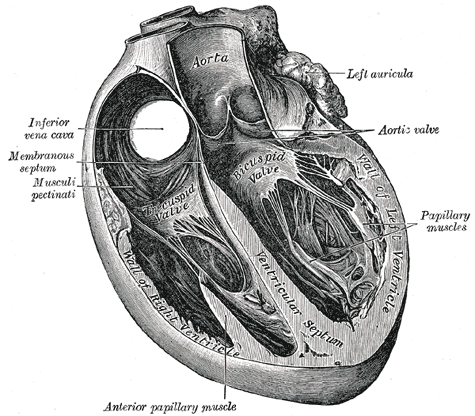
\includegraphics[width=0.7\textwidth]{figures/sample/Gray498.png} 
\caption[Four-chamber illustration of the human heart.]{Four-chamber illustration of the human heart.  Clockwise from upper-left: right atrium, left atrium, left ventricle, right ventricle.}
\label{fig:fourchamber}\end{figure}

The use of acoustic waves for medical diagnosis, inspired by naval sonar, was initially developed in the 1940s \cite{gagliardi_ultrasonography_1996}.  By 1954, the first clinically useful cardiac ultrasound -- examining motion of the mitral valve in stenosis -- was reported \cite{edler_ultrasonic_1957}.  These early scans were one-dimensional images (`A-mode'), sometimes repeated to generate a time axis (`M-mode').   The sector-scanning probe was developed in the 1970s \cite{bom_ultrasonic_1971,griffith_sector_1974}, leading to the `B-mode' that a modern cardiologist would recognise as an echocardiogram.



%% APPENDICES %% 
% Starts lettered appendices, adds a heading in table of contents, and adds a
%    page that just says "Appendices" to signal the end of your main text.
\startappendices
% Add or remove any appendices you'd like here:
\begin{savequote}[8cm]
\textlatin{Cor animalium, fundamentum e\longs t vitæ, princeps omnium, Microco\longs mi Sol, a quo omnis vegetatio dependet, vigor omnis \& robur emanat.}

The heart of animals is the foundation of their life, the sovereign of everything within them, the sun of their microcosm, that upon which all growth depends, from which all power proceeds.
  \qauthor{--- William Harvey \cite{harvey_exercitatio_1628}}
\end{savequote}

\chapter{\label{app:1-cardiophys}Review of Cardiac Physiology and Electrophysiology}

\minitoc

Appendices are just like chapters.  Their sections and subsections get numbered and included in the table of contents; figures and equations and tables added up, etc.  Lorem ipsum dolor sit amet, consectetur adipiscing elit. Sed et dui sem. Aliquam dictum et ante ut semper. Donec sollicitudin sed quam at aliquet. Sed maximus diam elementum justo auctor, eget volutpat elit eleifend. Curabitur hendrerit ligula in erat feugiat, at rutrum risus suscipit. Pellentesque habitant morbi tristique senectus et netus et malesuada fames ac turpis egestas. Integer risus nulla, facilisis eget lacinia a, pretium mattis metus. Vestibulum aliquam varius ligula nec consectetur. Maecenas ac ipsum odio. Cras ac elit consequat, eleifend ipsum sodales, euismod nunc. Nam vitae tempor enim, sit amet eleifend nisi. Etiam at erat vel neque consequat.

\section{Anatomy}
\label{sec:anatomy}

Lorem ipsum dolor sit amet, consectetur adipiscing elit. Donec accumsan cursus neque. Pellentesque eget tempor turpis, quis malesuada dui. Proin egestas, sapien sit amet feugiat vulputate, nunc nibh mollis nunc, nec auctor turpis purus sed metus. Aenean consequat leo congue volutpat euismod. Vestibulum et vulputate nisl, at ultrices ligula. Cras pulvinar lacinia ipsum at bibendum. In ac augue ut ante mollis molestie in a arcu.

Etiam vitae quam sollicitudin, luctus tortor eu, efficitur nunc. Vestibulum maximus, ante quis consequat sagittis, augue velit luctus odio, in scelerisque arcu magna id diam. Proin et mauris congue magna auctor pretium id sit amet felis. Maecenas sit amet lorem ipsum. Proin a risus diam. Integer tempus eget est condimentum faucibus. Suspendisse sem metus, consequat vel ante eget, porttitor maximus dui. Nunc dapibus tincidunt enim, non aliquam diam vehicula sed. Proin vel felis ut quam porta tempor. Vestibulum elit mi, dictum eget augue non, volutpat imperdiet eros. Praesent ac egestas neque, et vehicula felis.

Pellentesque malesuada volutpat justo, id eleifend leo pharetra at. Pellentesque feugiat rutrum lobortis. Curabitur hendrerit erat porta massa tincidunt rutrum. Donec tincidunt facilisis luctus. Aliquam dapibus sodales consectetur. Suspendisse lacinia, ipsum sit amet elementum fermentum, nulla urna mattis erat, eu porta metus ipsum vel purus. Fusce eget sem nisl. Pellentesque dapibus, urna vitae tristique aliquam, purus leo gravida nunc, id faucibus ipsum magna aliquet ligula. Lorem ipsum dolor sit amet, consectetur adipiscing elit. Proin sem lacus, rutrum eget efficitur sed, aliquam vel augue. Aliquam ut eros vitae sem cursus ultrices ut ornare urna. Nullam tempor porta enim, in pellentesque arcu commodo quis. Interdum et malesuada fames ac ante ipsum primis in faucibus. Curabitur maximus orci purus, ut molestie turpis pellentesque ut.

Donec lacinia tristique ultricies. Proin dignissim risus ut dolor pulvinar mollis. Proin ac turpis vitae nibh finibus ullamcorper viverra quis felis. Mauris pellentesque neque diam, id feugiat diam vestibulum vitae. In suscipit dui eu libero ultrices, et sagittis nunc blandit. Aliquam at aliquet ex. Nullam molestie pulvinar ex vitae interdum. Praesent purus nunc, gravida id est consectetur, convallis elementum nulla. Praesent ex dolor, maximus eu facilisis at, viverra eget nulla. Donec ullamcorper ante nisi. Sed volutpat diam eros. Nullam egestas neque non tortor aliquet, sed pretium velit tincidunt. Aenean condimentum, est ac vestibulum mattis, quam augue congue augue, mattis ultrices nibh libero non ante. Lorem ipsum dolor sit amet, consectetur adipiscing elit.

Aenean volutpat eros tortor, non convallis sapien blandit et. Maecenas faucibus nulla a magna posuere commodo. Nullam laoreet ante a turpis laoreet malesuada. Phasellus in varius sem. Vestibulum sagittis nibh sed tincidunt blandit. Donec aliquam accumsan odio sit amet lacinia. Integer in tellus diam. Vivamus varius massa leo, vitae ullamcorper metus pulvinar sed. Maecenas nec lorem ornare, elementum est quis, gravida massa. Suspendisse volutpat odio ex, ac ultrices leo ultrices vel. Sed sed convallis ipsum. Pellentesque euismod a nulla sed rhoncus. Sed vehicula urna vitae mi aliquet, non sodales lacus ullamcorper. Duis mattis justo turpis, id tempus est tempus eu. Curabitur vitae hendrerit ligula.

Curabitur non pretium enim, in commodo ligula. Etiam commodo eget ligula a lacinia. Vestibulum laoreet ante tellus, vel congue sapien ornare in. Donec venenatis cursus velit vitae pulvinar. Pellentesque habitant morbi tristique senectus et netus et malesuada fames ac turpis egestas. Suspendisse in metus lectus. Pellentesque gravida dolor eget finibus imperdiet. Duis id molestie tortor. Mauris laoreet faucibus facilisis. Aliquam vitae dictum massa, sit amet dignissim lacus.

Fusce eleifend tellus id ex consequat maximus. Donec ultrices ex ut turpis ornare, non molestie mi placerat. Nulla sit amet auctor nunc, sit amet euismod elit. Phasellus risus tellus, condimentum a metus et, venenatis tristique urna. Cras mattis felis eget ipsum fermentum egestas. Ut augue odio, venenatis id convallis vel, congue quis augue. Maecenas sed maximus est, posuere aliquet tortor. Ut condimentum egestas nisi eu porttitor. Ut mi turpis, posuere id lorem vel, elementum tempor arcu.

Morbi nisl arcu, venenatis non metus ac, ullamcorper scelerisque justo. Nulla et accumsan lorem. Mauris aliquet dui sit amet libero aliquet, in ornare metus porttitor. Integer ultricies urna eu consequat ultrices. Maecenas a justo id purus ultricies posuere sed et quam. Cum sociis natoque penatibus et magnis dis parturient montes, nascetur ridiculus mus. Sed eleifend risus quis aliquet gravida. Nullam ac erat porta est bibendum dictum in a dolor. Nam eget turpis viverra, vulputate lectus eget, mattis ligula. Nam at tellus eget dui lobortis sodales et ut augue. In vestibulum diam eget mi cursus, ut tincidunt nulla pellentesque.

Aliquam erat volutpat. Sed ultrices massa id ex mattis bibendum. Nunc augue magna, ornare at aliquet gravida, vehicula sed lorem. Quisque lobortis ipsum eu posuere eleifend. Duis bibendum cursus viverra. Nam venenatis elit leo, vitae feugiat quam aliquet sed. Cras velit est, tempus ac lorem sed, pharetra lobortis ipsum. Donec suscipit gravida interdum. Nunc non finibus est. Nullam turpis elit, tempus non ante.

\section{Mechanical Cycle}

Lorem ipsum dolor sit amet, consectetur adipiscing elit. Aenean tellus est, suscipit sed facilisis quis, malesuada at ipsum. Nam tristique urna quis quam iaculis, et mattis orci pretium. Praesent euismod elit vel metus commodo ultrices. Vestibulum et tincidunt ex, in molestie ex. Donec ullamcorper sollicitudin accumsan. Etiam ac leo turpis. Duis a tortor felis. Nullam sollicitudin eu purus ac hendrerit. Nam hendrerit ligula libero, eget finibus orci bibendum a. Aenean ut ipsum magna.

Ut viverra, sapien sed accumsan blandit, nisi sem tempus tellus, at suscipit magna erat ornare nunc. Proin lacinia, nisi ut rutrum malesuada, nibh quam pellentesque nunc, sit amet consectetur purus felis ac tortor. Suspendisse lacinia ipsum eu sapien pellentesque mattis. Mauris ipsum nunc, placerat non diam vel, efficitur laoreet nunc. Sed lobortis, ipsum eget gravida facilisis, sem nulla viverra mi, in placerat eros sem viverra lacus. Aliquam porta aliquet diam vel commodo. Nulla facilisi. Duis erat libero, lobortis vel hendrerit vitae, sagittis id dui. Nulla pretium eros nec quam tincidunt, vel luctus mi aliquam. Integer imperdiet purus in est tristique venenatis. Ut pellentesque, nunc vitae iaculis ultricies, urna turpis dignissim risus, a laoreet felis magna nec erat.

Quisque sollicitudin faucibus ligula, et egestas nibh dictum sit amet. Proin eu mi a lectus congue pretium eu quis arcu. Suspendisse vehicula libero eu ipsum aliquam, vel elementum nibh mattis. Sed sed sapien vitae turpis tristique pulvinar a ut metus. Etiam semper gravida est, mollis gravida est porta ac. Proin eget tincidunt erat. Maecenas ultrices erat eget purus ultricies, ut lacinia arcu dictum. Nam et nisi sit amet ex congue mattis vel eget lorem. Aliquam erat volutpat. Pellentesque porttitor nibh vitae elementum consectetur. Aenean et est lobortis, congue sapien non, ullamcorper sapien. Ut facilisis sem non dapibus vehicula.

Mauris euismod odio dolor, sit amet gravida mauris placerat et. Curabitur nec dolor non nibh molestie lobortis dignissim non ante. Nullam rutrum lobortis ultrices. Aenean ex erat, elementum sed maximus id, posuere id quam. Proin rutrum ex elit, pretium aliquam risus finibus at. Aenean egestas orci velit, sed aliquet sapien condimentum a. Duis consequat, arcu eu viverra venenatis, dolor lorem gravida lectus, non aliquet nisi sem at augue. Donec laoreet blandit luctus. Aenean vehicula nisl vel faucibus luctus. Sed ut semper velit, vitae laoreet magna. Sed at interdum magna.

Sed iaculis faucibus odio, eu aliquam purus efficitur vel. Cras at nulla ac enim congue varius ut et nulla. Integer blandit mattis augue.

\section{Electrical Cycle}
\label{sec:electcycle}

Lorem ipsum dolor sit amet, consectetur adipiscing elit. In faucibus condimentum rhoncus. Ut dictum nisl id risus gravida lobortis. Sed vehicula mollis tellus ut varius. Fusce eget egestas dui, et commodo dui. Proin sollicitudin interdum tempus. Nullam in elit a enim fringilla bibendum. Vestibulum sodales pellentesque condimentum. Nulla facilisi. Nunc et dolor in nulla eleifend dictum at vel ligula. Aliquam ut velit non elit ullamcorper porta ac et ex. Fusce ornare magna non nunc vestibulum, eget molestie quam dictum. In interdum aliquam odio, in posuere tellus convallis quis. Curabitur non diam elit. Proin vulputate orci diam, a tincidunt ante luctus eu. Ut a viverra ligula. Curabitur pulvinar tempus tellus eget suscipit.

Aliquam posuere massa at ante dapibus congue. Curabitur ullamcorper tortor eget consectetur aliquet. Mauris tempor magna id mauris fringilla, a varius erat blandit. Nam eleifend ullamcorper placerat. Phasellus augue tortor, volutpat bibendum lorem nec, fringilla volutpat nisl. Mauris cursus urna metus, vel eleifend orci iaculis ut. Sed sit amet scelerisque massa, quis consequat dui. Donec semper sem dui, ac placerat velit egestas vel. Nulla facilisi. Quisque tellus eros, sagittis malesuada augue ut, faucibus dictum nulla. Vestibulum non dapibus erat, ut consequat libero. Ut turpis mi, dapibus commodo libero lobortis, maximus vestibulum lectus. Vestibulum sit amet sapien dapibus, tincidunt leo in, suscipit arcu. Sed in erat bibendum, laoreet eros eu, pellentesque justo. Nulla sodales purus neque, eget maximus ipsum consequat at. Maecenas a nisl sagittis, tempus ipsum sed, dictum mauris.

Suspendisse posuere odio lacus, at auctor tortor vehicula sed. Phasellus suscipit ornare enim vitae placerat. Sed viverra purus vel sapien tempor, quis iaculis erat laoreet. Aenean vel nunc vestibulum, ornare nunc ac, mollis urna. Aenean ultrices felis ipsum, ac semper est ullamcorper in. Donec in justo varius, egestas tortor ut, venenatis augue. Duis mattis, ligula quis lacinia fringilla, tellus neque accumsan ipsum, vitae tempor metus elit vel nibh. Curabitur porttitor urna nec sapien tempor, et porttitor velit malesuada.

Suspendisse aliquam nisl quis placerat vulputate. Proin dapibus ipsum ac ante sagittis, volutpat auctor sem dapibus. Nam in facilisis odio. Integer ante mauris, eleifend et pulvinar in, venenatis quis ligula. Phasellus posuere sollicitudin tortor eget euismod. Maecenas mollis tortor eget justo vulputate sagittis. Etiam hendrerit massa quis ex molestie sodales. Quisque facilisis erat lacus, id convallis sem suscipit bibendum. Integer dui urna, pharetra sed porta sed, bibendum ut odio. Donec placerat at lectus egestas consequat. Sed id rhoncus est, vitae vulputate sapien. Fusce tempus quam lorem, id ornare turpis sodales sed. Integer aliquet urna eget condimentum consequat. Vestibulum quis dui vel ligula posuere luctus id nec turpis.

Nam vitae placerat lacus. Mauris scelerisque interdum volutpat. Nunc aliquet tristique enim, sit amet molestie felis ullamcorper vitae. Nullam sollicitudin orci orci, in condimentum tellus consectetur in. Nam id justo justo. Fusce eget finibus est. Proin id tortor nec quam cursus vehicula. Aliquam ultrices eros eros, a tincidunt elit eleifend auctor.

Nullam consectetur dapibus ligula sit amet efficitur. Nunc non posuere sapien. Vivamus dui nisl, aliquam id ipsum non, pulvinar ornare neque. Nunc rhoncus pretium congue. Fusce id laoreet enim. Cras sed massa in eros bibendum auctor in nec sem. Nam commodo, velit id porta consequat, mi arcu gravida lorem, ut aliquam elit ante quis dui. Quisque in massa sed nibh blandit dictum.

Vestibulum molestie consectetur porttitor. Donec tincidunt vel orci at pharetra. Nullam id felis sit amet nulla tempus lacinia. Integer egestas ullamcorper massa, ut ultricies diam congue sit amet. Cras sit amet velit at nibh vehicula finibus a et lorem. Cras odio metus, venenatis ut ultrices non, ornare ac orci. Morbi et nulla dui. Mauris dictum molestie nibh, eu efficitur lorem accumsan quis.

\section{Cellular Electromechanical Coupling}
\label{sec:electromech}

Lorem ipsum dolor sit amet, consectetur adipiscing elit. Nullam vitae consectetur metus, ac maximus ex. Quisque vitae ex eu lectus ultricies consequat vel non lorem. Etiam odio ipsum, tempus ut lobortis in, molestie ac leo. Vivamus mollis feugiat bibendum. Vestibulum eget venenatis quam. Aenean faucibus, massa sed ullamcorper porta, arcu nunc iaculis velit, quis consectetur purus neque placerat nibh. Vestibulum elit nunc, dignissim vulputate venenatis et, sodales non massa. Proin leo ligula, vehicula eu aliquam varius, posuere a dolor. Donec iaculis auctor neque, sit amet gravida libero porta vel. Vivamus consequat elementum lacus, at bibendum mauris egestas nec. Fusce fermentum diam eu dolor ornare, vitae vestibulum leo interdum. Morbi luctus libero quis dictum laoreet. Etiam semper porta ante, vel ullamcorper enim sodales quis.

Nullam eu nisi faucibus, fermentum ex auctor, tempor arcu. Phasellus condimentum erat mi, condimentum malesuada ligula congue venenatis. Nullam gravida imperdiet urna quis cursus. Ut tempus nec purus eget posuere. Cras non nulla sit amet justo aliquet pellentesque nec sed eros. Nam aliquam nisl urna, in placerat magna gravida venenatis. Donec interdum vel magna ullamcorper molestie. Nunc felis neque, rhoncus fringilla faucibus sit amet, ultrices sed magna. Maecenas malesuada hendrerit diam in ultrices. Nam libero urna, volutpat ut auctor eget, interdum sed odio. Vestibulum suscipit mauris nec augue ornare, ut eleifend nulla gravida. Proin imperdiet, mauris quis consectetur porta, leo dui convallis leo, id lobortis massa diam eu libero. Aenean hendrerit vel ante aliquam venenatis. Pellentesque bibendum pretium odio, ut sagittis lectus feugiat a. Donec porttitor vulputate lacus.

Nunc volutpat efficitur lacus in aliquet. Nullam non iaculis diam, at ultrices diam. Proin vehicula vulputate cursus. Morbi tempus sapien id urna lobortis interdum. Maecenas elementum sagittis elementum. Donec at sodales velit, a posuere tortor. Nulla id hendrerit tortor. Sed semper velit in magna sagittis pulvinar. Nulla nec arcu molestie, ultricies sapien sit amet, sollicitudin nisi. Donec nisi massa, suscipit ut dignissim quis, lacinia id leo.

Suspendisse ut mi metus. Morbi tincidunt ligula in porttitor consectetur. Integer eu urna urna. Suspendisse potenti. Mauris sit amet felis eu diam auctor ullamcorper. Morbi in porta nisi. Nam ante tortor, venenatis vitae tempor sed, sagittis vitae velit. In semper orci sit amet nisi ullamcorper varius. Aenean dignissim ultrices imperdiet. Maecenas lacinia enim id neque porttitor iaculis. Curabitur laoreet ante ut urna dignissim, id sollicitudin metus consectetur. Aenean massa ipsum, auctor vel ante vel, blandit dignissim libero. Fusce interdum ac magna et interdum.



%%%%% REFERENCES

% JEM: Quote for the top of references (just like a chapter quote if you're using them).  Comment to skip.
\begin{savequote}[8cm]
The first kind of intellectual and artistic personality belongs to the hedgehogs, the second to the foxes \dots
  \qauthor{--- Sir Isaiah Berlin \cite{berlin_hedgehog_2013}}
\end{savequote}

\setlength{\baselineskip}{0pt} % JEM: Single-space References

{\renewcommand*\MakeUppercase[1]{#1}%
\printbibliography[heading=bibintoc,title={\bibtitle}]}


\end{document}
